\subsection{Implementation}

The algorithm computational load and complexity is discussed in this section. The implementation realized in this thesis is described in figure \ref{fig:systemimplementaiton}, there exist methods to improve the efficiency of the algorithm but this is not the focus of this work. \footnote{Dmochowski and Benesty \cite{dmochowski2007generalized} present a method which improve the full map search}. First of all the delays across the microphones for each search location are computed in advance, stored in memory and fed to the algorithm which correspond to the "Compute array delays" system block therefore this will not cound as computational load. Note that value of the cross correlation between each pairs of microphones are computed upfront to avoid the computation of the cross correlation in the search loop. This step is the GCC-PHAT system box. The SRP system box related to the steering of the array response to the search location $(\tetha,\phi)$, this step beamforms each microphones pairs to the search position and output each pair power ($P_{all}$). The minimum power then select the minimum power of all the pairs and maps it to the search location.

\begin{figure}[!ht]
    \centering
    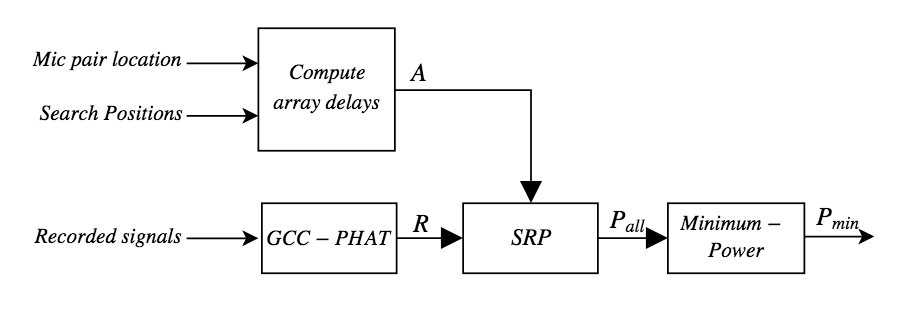
\includegraphics[width=1\textwidth]{Figures/system1.png}
    \caption{Overall localization algorithm}
    \label{fig:systemimplementaiton}
\end{figure}

The minimum power SRP-PHAT algorithm combines beamforming techniques with cross correlation methods for several pairs of microphones. While the beamforming part is not depending on the size of the input data, it might become a challenge memory wise. Delay of the array are precomputed in advance and store into a memory. The most demanding part of the algorithm is definitely the cross correlation part. By performing the cross correlation in the frequency domain, i.e by using the cross spectrum between pairs of microphones, better averaging of the stationary sources are obtained as well as best efficiency compare to time domain  cross correlation ($\mathcal{O}(n^2)$). The cross spectrum is described in the figure \ref{fig:crossspectrumsystem} 

\begin{figure}[H]
    \centering
    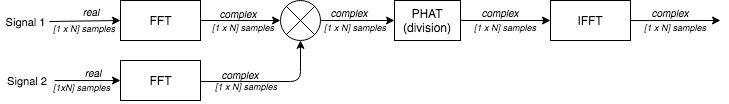
\includegraphics[width=1\textwidth]{Figures/crossspectrum3.png}
    \caption{Cross spectrum between two signals}
    \label{fig:crossspectrumsystem}
\end{figure}

Dmochowski and Benesty \cite{dmochowski2007generalized} detailed the number of computation needed for the GCC-PHAT part, and the worst-case complexity of the cross spectrum system is listed below with n the number of input sample in the algorithm . 

\begin{center}
  \begin{tabular}{ |c | c | }
    \hline
    Operation  & Worst-case Complexity \\ \hline
    FFT  & $\mathcal{O}(n\log{}n)$  \\ \hline
    Complex Multiplication  & $\mathcal{O}(n)$  \\ \hline
    PHAT (Division)  & $\mathcal{O}(n)$  \\ \hline
    IFFT  & $\mathcal{O}(n\log{}n)$  \\
    \hline
  \end{tabular}
\end{center}

The SRP block is the part of the algorithm taking more time however it does not scale with the number of sample but rather with the number of delay to look up in the algorithm. Dmochowski and Benesty \cite{dmochowski2007generalized} also proposed a more efficient way to perform the SRP. Therefore the overall algorithm complexity is scaling with the FFT complexity $\mathcal{O}(n\log{}n)$ when n is the number of sample however when n is small the FFT is negligible to the number of delay lookups. 
%Table \ref{tab:extime} gives a measure of the execution time of the minimum SRP-PHAT script. 

%\begin{center}
%  \begin{tabular}{ c | c | c |}
%    \cline{2-3}
%    \multicolumn{1}{c|}{} & \multicolumn{2}{ c| }{Execution time} \\ \cline{2-3}
%    \hline
%    \multicolumn{1}{|c|}{signal lengths (seconds)}   & thinkpad i5 & Macbook 2012  \\ \cline{1-3}
%    \multicolumn{1}{|c|}{10}  &  &    \\ \cline{1-3}
%    \multicolumn{1}{|c|}{100} & &     \\ \cline{1-3}
%    \multicolumn{1}{|c|}{1000}  & &   \\
%    \hline
%  \end{tabular}
%  \label{tab:extime}
%\end{center}

Memory wise, the function computing the delay at each pair of microphones in the array can be expensive depending on the localization resolution used and the number of microphone pairs. For 1$\degree$ resolution is used $360*180=64800$ delays are computed for a pair of microphones. For 6 microphone pairs,$360*180*6=388800$.  Using type float64 (8 bytes), the delay table is  $360*180*6*8=3110400$ = 3.11 MB. However if high resolution is needed, i.e 0.1$\degree$ resolution $3600*1800=6480000$ delays are computed. For 6 microphones,$3600*1800*6=38880000$.  Using type float64 (8 bit), the delay table is  $3600*1800*6*8=311040000$ = 311.04 MB.


